\chapter{Discount Spaceship}

\begin{wrapfigure}{O}{\figwidth}
	\begin{center}
		
\includegraphics[width=\figwidth]{pics/7/1.png}
	\end{center}
\end{wrapfigure}
The squad is getting a tour of the impressively large shuttle they’ve just boarded from none other than their former squadmate Nubby. 
Last they’d seen him, he’d been reassigned to quartermaster duties after his legs were removed by a treacherous Interrogator. 
Now he’s happily stomping around on a pair of augmetic legs while proudly explaining how he’s the mission’s “supply officer”. 

This announcement is being met with considerable skepticism by Sarge, who is the only member of the squad actually listening.

Doc is paying far more attention to Nubby’s shiny new metal legs and is interrupting the rambling tour with questions about how they’d been attached. 
When Nubby doesn’t provide any helpful answers Doc asks Sarge to hold the little trooper up so he can take a look.

Meanwhile Twitch’s curiosity and paranoia are driving him to find out just what is inside all the large metal containers being loaded onto the shuttle. 
Cutter, who found the lack of sword-related topics in the tour incredibly boring, is helping the demolitions trooper by prying open one of the boxes. 
When the lid finally pops off, both guardsmen jump back and start swearing.

Doc and Sarge, who is still holding Nubby up by the shoulders, come over to see what the matter is. 
When Sarge sees what’s inside the container as well as the identical markings on all the other containers, he starts shaking the suspended guardsman angry terrier.

\greentext{>>“NUBBY! Just why the hell are we taking a few thousand servitors with us?”}

\greentext{>The All Guardsmen Party Buys A Spaceship}


\begin{wrapfigure}{O}{\figwidth}
	\begin{center}
		
\includegraphics[width=\figwidth]{pics/7/2.png}
	\end{center}
\end{wrapfigure}
So no shit there we were, on a shuttle filled with tech-priests and an army of servitors, on our way to assist in the purchase an entire warp-capable starship for our Inquisitor. 
Not a normal space transport, not a shuttle, not a flier, but an entire damned warpship; 
the smallest of which were typically over a kilometer long and worth more than a dozen regiments of Guard. 
And to top it all off, Nubby Nubbs was standing there, proud as anything, telling the rest of us that HE was in charge of the operation. 
It  was completely unbelievable.

To clarify, it wasn’t unbelievable in the sense that we couldn’t fathom how the universe could be so strange and cruel, we literally didn’t believe a word Nubby had said. 
No one with a scrap of intelligence would send him out to buy the recaff, much less a bloody warpship. 
Sure, we’d all trust Nubby at our back in a firefight any day, but the man was a petty thief, a compulsive liar, and had actually been mistaken for a gretchin on more than one occasion. 
Sarge told the trooper to stuff a sock in it, and we all went to get a more realistic briefing from the tech-priests that were coming with us.

There seemed to be a lot of cogboys on the big cargo shuttle with us; 
every room or hallway was filled with creepy metal men squawking at each other in binary. 
We found the one that Oak had implied was the head tech-priest in a conference room surrounded by a bunch of subordinates. 
He was obviously holding some sort of conference or briefing, but we couldn’t understand any of their robotic chatter. 
Sarge just stood there awkwardly, and then started loudly clearing his throat until a few cogboys were waved away to deal with us.

\begin{wrapfigure}{O}{\figwidth}
	\begin{center}
		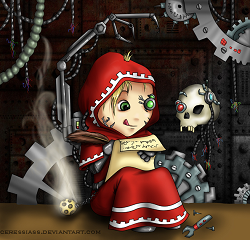
\includegraphics[width=\figwidth]{pics/7/3.png}
	\end{center}
\end{wrapfigure}
That became an annoying trend over our journey; 
the head tech-priest and his senior flunkies would never talk to us directly. 
We were sure they could understand gothic, but they just never seemed to speak in anything but their damned machine language. 
Every time we needed to talk to one of them a junior cogboy would be called up to act as a translator or lead us away so we didn’t disturb the senior techies. 
This did not endear them to us, and we didn’t go out of our way to treat them any better. 
We did get pretty familiar with the junior tech-priests though.

Well not exactly familiar, there were a bunch of them and it was damned hard to pick out which pile of metal tentacles was Brother Ticinius and which was Brother Cacistus. 
Woe betide the poor guardsmen who mistook Logis Guminnio for Constructor Periphanes. 
Such a mistake was incredibly insulting and a clear indication of our inferior intellect. 
Matters were not helped by their damned tendency to switch out their augmetics; 
just when you got used to Arch-Brother-Lexi-Mechanic Cogitus Boyus being the tall bastard with the heavy duty servo-arm, he’d swap it out for some sort of sparky tentacle job and replace his legs with treads or something. 
We would have gone crazy if it weren’t for the two lowest ranking tech-priests in the bunch, tech-acolytes Jim and Hannah.
 
The two acolytes were the most junior tech-priests on the mission and were obviously the Mechanicus equivalent of the Regimental Gofer. 
Every time you saw them they’d be carrying something, moving as fast as possible without running, or covered head to toe with grease and other less pleasant fluids. 


We liked Jim and Hannah: 
they were practically kids, had most of their original parts, and you could pronounce their names while drunk. 
Best of all, they had a weary put-upon attitude which warmed the khaki colored blobs which passed for our souls. 
We quickly made them honorary Guardsmen and began taking all of our questions to them.

\begin{wrapfigure}{O}{\figwidth}
	\begin{center}
		
\includegraphics[width=\figwidth]{pics/7/4.png}
	\end{center}
\end{wrapfigure}
Once we met Jim and Hannah, we were finally able to get the real details of our mission. 
The gist of it was that the tech-priests and our squad were all being sent to discreetly purchase a second hand warpship. 
Presumably so it could be used to carry around Oak’s recruitment teams without causing a fuss.

To our collective relief the acolytes confirmed that Nubby was not in charge of the operation. 
He was merely there to act as the public face for the purchase and general observer. 
His superiors in supply had already chosen the ship, negotiated a price range, gotten the funds into place, hired a navigator and astropath, and handed Nubby a very explicit set of orders. 


The head Magos and the other tech-priests would handle everything else, and be more or less in command from the second the ship was deeded over and the original crew was evicted. 
They’d do the inspection, prep the ship for travel, and perform any repairs. 
Finally, once the priests deemed the ship ready for travel, they’d use their servitor army to fly the whole damned thing back to some secret Inquisition shipyard for a refit.

This all made sense to us, but it was still a wonder that Nubby had been chosen for any part of this mission. 
He insisted that his superiors had recognized his "'Quisition skills an' persnal 'sperience wif ships like dis," not to mention his "cleva' negotiashun tactics" and "cunnin' merkantile mind." This was bullshit and we all knew it. 
To a man the rest of us believed that he’d been sent because no one would ever look at him and think "Inquisitorial Agent." 

The rest of us were there to act as backup for Nubby. 
Officially this was because every procurer in the field was supposed to have a bunch of trustworthy and discreet agents to assist them. 
At first we wondered just why we had been chosen over other available agents, but after we figured out why Nubby had been sent it was plain as day why we were sent. 
Obviously our squad had been chosen because we all looked like the sort of incompetent ex-guard goons that a complete cretin would employ as bodyguards. 
Thanks Oak.

\begin{wrapfigure}{O}{\figwidth}
	\begin{center}
		
\includegraphics[width=\figwidth]{pics/7/5.png}
	\end{center}
\end{wrapfigure}
Now we’d traveled a fair bit during our careers in the Inquisition, but this trip was something else. 
This time we didn’t have our own quiet section of ship. 
Instead we were surrounded by dozens of cogboys running around preparing an army of servitors for crewing a warpship. 
Everywhere you went there’d be tech-priests chattering at each other, chanting and lighting incense, welding random pieces of metal, or doing incredibly unsettling things to their servitors.

The ship itself was some sort of Mechanicus transport, and the quarters available made us all think wistfully of the berths the Rupert had gotten for us. 
Apparently when you become a full tech-priest you stop desiring beds fancier than a wide metal shelf or food that actually has flavor. 
Also Mechanicus toilets can best be described as “Terrifying.”

We all tried to stay out of the way and keep to ourselves, but it just didn’t work. 
We always seemed to be underfoot or under tread or under antigrav skimmer. 
There simply wasn’t room for anyone that wasn’t part of whatever mad plan the techies were all following. 
Cargo haulers would bull through us during morning PT, random tech-priests would shout at us if we touched or sat on anything, and our quarters were randomly repurposed for storage, sometimes while we were still in them. 
No man should wake up in a dark room surrounded by thirty deactivated servitors.

None of us were happy, but Twitch had the worst of it; 
he just couldn’t function well without a secured perimeter. 
We were about ready to outright fortify a cargobay and try to hold it against the cogboys, when Doc got his idea. 
He suggested that the only way to survive the trip was to become "part of the pattern."

We spent the rest of the voyage following Jim and Hannah around like lost puppies. 
We slept when and where they slept, we ate when they ate, and we did our best to help with whatever unpleasant task they were working on. 
We probably weren’t very helpful, but it kept us alive and relatively sane.

\begin{wrapfigure}{O}{\figwidth}
	\begin{center}
		
\includegraphics[width=\figwidth]{pics/7/6.png}
	\end{center}
\end{wrapfigure}
It was an immense relief when we finally reached our destination. 
We piled onto a shuttle and rode to a local orbital station where a few scribes were waiting to brief us on the purchase. 
We blew them all off and slept for about twenty hours in the blissful quiet of our cogboy-free rental rooms.

The briefings and preliminary negotiations took about a week, and aside from Nubby none of us really had to do anything. 
We more or less hung out in hallways while various scribes became incredibly frustrated with Nubby. 
There were no assassination attempts, no cultists infiltrators, no ork kommando raids, and certainly no genestealers attacks. 
Just a bunch of boring guard duty while Nubby drove various expensive lawyers and financial experts into a state of incoherent rage. 
One of them did actually try to kill him, but since Nubby had just stolen the man’s wallet it was perfectly understandable.

We did pay a little attention to what was going on; 
guard duty was boring and they weren’t really hiding the documents or diagrams. 
Most of it was legal gibberish, ancient trade logs, and figures about engine strength and storage capacity. 
None of which we even tried to understand, but there were some nice pictures. 
From what we saw the ship was a small one, only two kilometers long, and was rather plain looking. 
Just the sort of ship for traveling around unnoticed.

The negotiations continued and some of the tech-priests were sent over to inspect the ship. 
They took a while, but confirmed that the ship "met all requirements." That done with, all that was left was the final meeting between Nubby and the current owner of the vessel.

\begin{wrapfigure}{O}{\figwidth}
	\begin{center}
		
\includegraphics[width=\figwidth]{pics/7/7.png}
	\end{center}
\end{wrapfigure}
Some fancy rooms were rented out for The Deal, and Nubby was crammed into a frilly suit complete with powdered wig. 
It was probably supposed to make him look like a dashing Imperial nobleman, but it really just made him look like a gretchin in a dress. 
It was hard not to laugh as we followed him to the meeting, and when we saw the man selling the ship it became nearly impossible.

If Nubby was a gretchin in a dress, then the seller was a giant squig in a suit. 
 The man was practically spherical, comically clumsy, and honked like a goose when he talked. 
He radiated an aura of incompetence and was followed by a cadre of thugs who all had the same suffused expressions we did.

The worst part was that the man obviously thought of himself as a Rogue Trader, and tried to dress the part. 
He must have gone through some catalogue and ordered one of everything. 
He had the gaudy coat with epaulets, the large hat with a feather in it, the cane that obviously contained a sword, and just to top it off, there was a cybernetic parrot perched on his shoulder. 
The problem was that while most Rogue Traders ooze confidence and danger, this one just oozed. 
We’d seen, fought, and redecorated a bathroom with the head of a real Rogue Trader before; 
this guy was more like a kid playing dress-up.

We just barely managed to keep our faces straight while Nubby and the wannabe greeted each other. 
Both of them were handed the relevant documents by their scribes and headed into a private room to complete the deal. 
The second the door had closed behind them, the fat man’s guards cracked up and we did likewise. 
It was just too much to bear. 
Both sets of scribes just shared a miserable look and settled down to wait.

The meeting took a surprisingly long time, and we all started to get nervous. 
Every part of the deal had been been hammered out beforehand, and this just supposed to be a matter of signing off. 
Emperor only knew what Nubby was getting up to in there. 


\begin{wrapfigure}{O}{\figwidth}
	\begin{center}
		
\includegraphics[width=\figwidth]{pics/7/8.png}
	\end{center}
\end{wrapfigure}
Neither of them hit their panic buttons though, so we sat tight and eventually both men came out alive and relatively well. 
Nubby had a disturbingly smug look and the seller seemed rather flustered, but both of them insisted that everything was sorted out. 
The scribes did a final review of the signed documents, got into a brief whispered argument with Nubby and the fat man, and then loudly confirmed that everything was in order. 
The seller’s scribes said that all of their men would be off the ship within thirty hours, and the whole party made a rather hasty exit.

That done with, we headed back to our quarters and passed the word on to the tech-priests. 
The cogboys confirmed that they were ready to board the ship and take over as soon as the former crew was out of the way. 
From there on out it was entirely their mission; 
we were just passengers and observers. 
All our squad had to do was keep out of the way until we arrived at the shipyard and someone came to collect us.

The tech-priests told us to stay in our quarters until they had their servitors in place, so we finished our business with the scribes, settled in for a few days of relaxation on the station, and asked Nubby about what had happened during the meeting. 
According to him the former captain had been a terrible negotiator and was easily haggled down. 
The little bugger was smug as hell about the whole thing and expected a big thank you from Oak for saving him a few billion thrones. 
None of us really believed him, Nubby was always full of that sort of shit, but the scribes were happy so it wasn’t really our problem. 
In retrospect not grilling Nubby and finding out exactly what sort of deal he got, or how he managed to get it, was a tremendous mistake.

\begin{wrapfigure}{O}{\figwidth}
	\begin{center}
		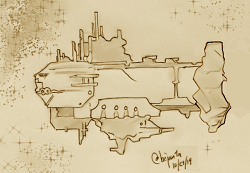
\includegraphics[width=\figwidth]{pics/7/9.png}
	\end{center}
\end{wrapfigure}
A few days of idleness later a shuttle was sent for us, and we were taken to the newest addition to Oak’s fleet, the Free Trader Occurrence Border.

As we approached the ship everyone clustered around the windows to get a good look at our purchase. 
A lot of things about the Occurrence Border grabbed the eye. 
There were the massive tanks for hauling fluids, the impressive arrays of docking hatches along the cargo bays, the odd variations in the color and design of the hull, but mostly there was the fact that the ship was about half as long as the diagrams said it should be.

It was amazing really. 
The Occurrence Border mostly followed the standard Imperial ship design; 
large engines in the tail, control tower rising above the rear of the ship, long and slightly skinny body. 
Except the bow was completely gone. 
The ship just ended half way through the body in a giant patchwork of scrap metal. 
It looked like someone had grabbed the ship, cut it with a giant cleaver, and then smashed the ragged edge flat. 
As one we all turned to look at Nubby; 
who muttered something about “good value for cost” and tried to sidle away.

It took a lot of shaking and yelling to get all the details out of Nubby. 
Apparently, well, the front fell off. 


The entire front of the vessel, a two kilometer warp-capable ship, which we had just purchased for a staggering amount of money, on behalf of the bloody Inquisition, Fell. 
Off.

He said it doesn’t happen often, just a sort of occasional time to time thing, overall its a very safe ship. 
In fact in the whole lifetime of the ship it only happened once, or twice, well maybe three times, definitely no more than four, but the important thing was that it wouldn’t ever happen again. 
The previous captain had fixed the problem for good by installing the “special made custom prow” after the last incident.

We all eyed the mushroom-shaped pile of slagged scrap on front of the ship and contemplated just what Oak would do to us. 
It would probably involve an excruciator and an airlock.

\begin{wrapfigure}{O}{\figwidth}
	\begin{center}
		
\includegraphics[width=\figwidth]{pics/7/10.png}
	\end{center}
\end{wrapfigure}
The rest of flight was split between yelling at Nubby and staring at the ship with a sort of morbid curiosity. 
The closer we got the more the imperfections became apparent: 
there were scars and burns, holes and gouges, and the most bizarre set of repairs and additions imaginable. 
The entire ship must have been stripped off and replaced with spare parts one piece at a time until nothing of the original was left visible. 
It was a wonder that the thing flew at all. 
Doc suggested that we might not get yelled at by Oak for any of this, because there was no way we’d survive the warp voyage home in this hulk.

Eventually the shuttle docked, and we walked into one of the Occurrence Border’s more intact cargo bays. 
Hannah the cog-girl was waiting there to guide us to our quarters. 
She led us through a maze of tunnels and gave us a rundown of situation on the way. 
Most of the servitors were in place, the navigator and astropath were on board, and the last few repairs and calibrations would be made during the trip. 
After a while Sarge cautiously asked her what the tech-priests thought about the state of the ship; 
her response surprised us.

She cheerily informed us that the entire vessel was an abomination in the eyes of the Omnissiah and “perfectly met all requirements”. 

That second part was a little confusing, but according to her the whole point was to acquire a thoroughly disreputable vessel that was still capable of running. 
The cogboys didn’t care if half the hull was missing, if the cargo bays leaked atmosphere, or if most of the ship was pieced together from old wrecks. 
As long as it could travel through the warp they were happy. 
After all, they were just here to take it to the shipyard; 
the priests there were the ones who would be refitting it for Inquisitorial use.

Nubby perked up at this, but Sarge reminded him that, even if the tech-priests were happy, the people who were paying for the ship and its refit probably wouldn’t be.

\begin{wrapfigure}{O}{\figwidth}
	\begin{center}
		
\includegraphics[width=\figwidth]{pics/7/11.png}
	\end{center}
\end{wrapfigure}
As we walked, all of us noticed dozens of papers fixed to panels, doors, controls, and such. 
At first we thought they were the usual purity seals or Mechanicus prayers, but then Twitch stopped and actually read a few. 
Each one said something like “This control panel governs the flow of plasma through bays D3-S15, no one remembers why we have plasma going through there, but if you shut them off engines 3 and 7 stop working,”  “The gravity in this corridor is tilted 37 degrees to the left,” and “Do not ever touch this button”. 

That last one showed up a lot.

When we asked Hannah about the notes, she lowered her voice and advised us to take them very seriously. 
They must have been left by the former crew and were incredibly helpful, but we were never to mention them to any of the more senior tech-priests. 
The cogboys were trying to ignore them since they didn’t need advice from anyone outside the priesthood, but unfortunately the notes were far more accurate than their own scans. 
The senior priests were taking it as a personal insult every time they had to refer to one of the notes to fix a problem. 
We all chuckled at that and promised to read any notes we came across.

Eventually we arrived in a cluster of rooms that Jim the acolyte was clearing out with the help of a bunch of servitors. 
He suggested that these would make good quarters, pointed us towards a storage closet with some relatively edible rations in it, handed us a data slate with a crude map of the ship, and recommended that we stay out of the way of the servitors and tech-priests. 
Once we were settled the two acolytes scampered off to their next task.

Sarge booted up the data slate, and, about ten seconds after Jim and Hannah had disappeared into the giant maze of metal that was our ship, we realized that none of us knew how to read a three dimensional map. 
The ensuing argument over whose job it had been to check the map earlier and what we were going to do now, was interrupted by the ship’s speakers blaring to life. 
There was a painful burst of binary followed by a monotone voice telling all hands to prepare for warp transit; 
then the universe went “glorp” and tasted like the color purple for a second.

\begin{wrapfigure}{O}{\figwidth}
	\begin{center}
		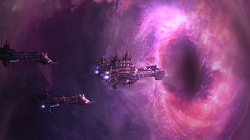
\includegraphics[width=\figwidth]{pics/7/12.png}
	\end{center}
\end{wrapfigure}
The one good thing you could say about the situation was that no one was trying to kill us, at least not on purpose anyway. 
On the other hand, we were cruising through the warp in a twisted heap of scrap held together with tape and spit, and none of us even knew where in the ship we were or how to read our map.

Now being lost is a long standing Guard tradition, but this was ridiculous. 
It’s hard enough to navigate in two dimensions with an accurate map and a directional finder. 
Three with an unreadable map and no way to tell which way you’re facing is just unfair. 
Without the ration bars we might have actually starved to death in our own ship, or at least been reduced to hunting the servitors for food.

After our quarters were secured we started trying to track down one of the tech-priests. 
We wanted to know where everyone else was, what was going on, and how the hell to read our map. 
Our comms didn’t work for shit inside all of this metal, and we didn’t have access to the ship’s communication system, so our search had to be done the old fashioned way: 
on foot with hand-drawn maps and trail markers. 


We didn’t feel like passengers on a ship. 
It was more like we were a recon force plotting hostile terrain, and boy was the terrain hostile. 
There were gravity shifts, depressurized sections of ship, exposed power conduits, rooms filled with hot plasma, and dozens of other hazards; 
only those helpful little notes kept us alive. 
Still, even though everything they said was helpful, the notes themselves were a bit disconcerting. 
They tended to be a little too precise, and Twitch swore that more of them were appearing in areas we’d already been through.

\begin{wrapfigure}{O}{\figwidth}
	\begin{center}
		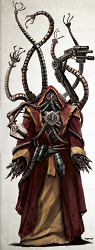
\includegraphics[width=\figwidth]{pics/7/13.png}
	\end{center}
\end{wrapfigure}
Doc was leading the patrol that found the first tech-priest. 
Unfortunately he refused to speak to us and ducked through a hatch which locked behind him; 
the second priest we found wasn’t give the chance. 
Doc and Nubby covered the exits while Cutter tackled the cogboy. 
Holding someone at gunpoint and asking them for technical support and directions probably isn’t the officially sanctioned way of doing this sort of thing, at least not when they’re on your side, but damned if it didn’t work well. 
The conversation was a little awkward though, the tech-priest turned out to be one of the ones who had briefed us during the trip out and was perfectly willing to talk to us. 
We did apologize.

Once we learned how to use the map we realized it was mostly empty space, but it did cover most of the important parts of the ship. 
It mapped out some of the bigger loading bays, the quarters the techies were using, the locations of several critical systems, and the giant spinal shipping corridor and freight lifts that most of the servitors used. 
The best part was that the terrified tech-priest showed us how to fill in the blank spots and add notes, which meant that we no longer had to depend on Doc’s hand drawn maps to get back to our base. 
Not that Doc was a bad artist mind you, he just had a little trouble figuring out how to draw a corridor that angled up and left while its gravity shifted to the right wall.

With the map in hand, our recon patrol released the tech-priest to go grease servitors or whatever and went off to find the two helpful techies. 
The rough plan was to get a hand with the comms situation from the acolytes, but unfortunately they weren’t in the quarters indicated on the map. 
Doc was dithering about whether to keep searching or wait for them to return, when Nubby suggested getting them to come to us. 
Based on our past experiences, Nubby argued, if we just annoyed enough of the senior tech-priests or started breaking things one of the acolytes would be sent to deal with us. 
Doc watched in horror as Nubby and Cutter went to work, but he didn’t actually do anything to stop them.

Three gutted cogitator terminals, two corridors flooded with coolant, another filled with less pleasant substances, and a dismembered maintenance servitor later, Sarge’s combead came to life. 
An exhausted sounding tech-acolyte Jim asked him to come pick up his team before someone killed them.

\begin{wrapfigure}{O}{\figwidth}
	\begin{center}
		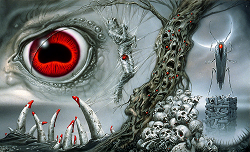
\includegraphics[width=\figwidth]{pics/7/14.png}
	\end{center}
\end{wrapfigure}
We still couldn’t use the ship’s comms, the acolytes said it was restricted to the priests for some techy reason, but our combeads were being boosted by the larger system. 
Combined with the functioning map and Jim and Hannah’s personal contact codes we had everything we needed to survive the rest of the trip, so we all went back to base to get a night’s sleep. 
Well if not a night’s then at least a solid ten hours worth: 
the ship’s light system seemed to be on several different clocks, and the ones in our quarters dimmed on a three hour cycle. 
Twitch eventually shot them out, and we just used our own lamps.

Now just to be clear, no one in the squad was a sissy and none of us had ever had trouble with warp travel before. 
We’d all faced down some incredibly weird and scary shit during our time in the Guard, not to mention what we’d seen as Inquisitorial goons. 
Our nerves might not have been made of steel, but they were definitely iron or possibly some good quality bronze. 
That said, the nightmares we had that night were fbloody terrifying. 
They were the sort of nightmares that take your every fear and failing and rub them in your face while you struggle to wake up and tell yourself it’s all a dream. 
We all woke up covered in sweat when one of Twitch’s perimeter alarms went off.

We didn’t even check what set off the alarm, all of us just sat there and thanked the Emperor for Twitch’s paranoia. 
After a few minutes Doc got up and pulled a yellow note off the inside of our door. 
It said “In case of bad dreams check Gellar Field integrity.”

The note had not been there when we went to sleep. 
 

\begin{wrapfigure}{O}{\figwidth}
	\begin{center}
		
\includegraphics[width=\figwidth]{pics/7/15.png}
	\end{center}
\end{wrapfigure}
While the note’s sudden appearance was mysterious as hell, none of them had steered us wrong so far and this one was pointing us towards what might be a very serious problem. 
On the list of incredibly horrible things that can go wrong during warp transit “Gellar Field Failure” is pretty much at the top. 
The Gellar Field Generator is literally the “anti-getting devoured by daemonic horrors” device; 
it is rather important that it keeps performing that function at all times while travelling through the warp.

The squad kitted up while Sarge commed Jim and asked nicely if he’d heard about anything about problems with the Gellar Field. 
We all watched as Sarge’s face started turning white, then red, then purple. 
We bailed out of the room just ahead of the explosion of rage and even through the sealed hatch we heard Sarge taking out a lot of frustration on poor Jim. 
The high points included:
\greentext{>“WHAT DO YOU MEAN WHICH ONE?” }

\greentext{>“WHY ARE THERE SIX?” }

\greentext{>“WHO IN THEIR RIGHT MIND WOULD INSTALL A DAMAGED GELLAR FIELD GENERATOR?”}

\greentext{>”WHO IN THEIR RIGHT MIND WOULD INSTALL SIX DAMAGED GELLAR FIELD GENERATORS?”}

\greentext{>”NO, THERE IS NOT A DIFFERENCE BETWEEN DAMAGED AND REFURBISHED!”}

\greentext{>“WHAT DO YOU MEAN IT WAS IN THE TECHNICAL BRIEFING? WHAT BRIEFING FOR WHO?”}

\greentext{>"WHERE'S NUBBY? I'llKILLSTRANGLEMURDERTHATLITTLEBASTARD GOODDEALI'LLSHOWHIMAGOODDEAL!"}


At that point Sarge burst through the hatch and Nubby decided it was a good time to go check what had set off the outer perimeter alarm while the rest of us restrained the irate noncom.

\begin{wrapfigure}{O}{\figwidth}
	\begin{center}
		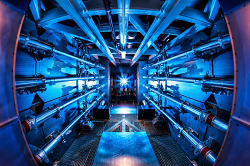
\includegraphics[width=\figwidth]{pics/7/16.png}
	\end{center}
\end{wrapfigure}
Eventually we got Sarge calmed down enough to speak coherently and he explained the whole messed up situation to us. 
Apparently the ship’s Gellar Field had been scrapped and replaced by several smaller models that had been scavenged from Emperor-knows-where. 
There were three along the length of the ship, one near the bridge, and two covering the top and bottom decks. 
We were currently near the one in the bow and from the look of things it was on the fritz. 
Jim said he’d take a look at it and suggested that we move our quarters farther back into the coverage of one of the other generators.

That sounded like a good idea, but we decided to take it a step further. 
We weren’t just going to find some random rooms in the next section of ship, we were going to hike our asses down to that Gellar Field Generator, set up camp, and bloody well sleep on it. 
There was not going to be any screwing around with this nightmare business. 
Sacktime is practically sacred and anything that disturbs it must be immediately dealt with; 
a guardsman who can’t fall asleep the second the perimeter is secure is not a true guardsman.

We packed up our quarters; 
rations, field gear, traps, munitions, everything we had was coming with us. 
As Twitch pulled down his perimeter defenses he found the triggered alarm tucked away in the side of a corridor with a note that said “Please do not obstruct the corridors”. 

That was a little disconcerting, but was something we could worry about later.

The hike aft went pretty quickly after we navigated up to the big spinal corridor, it really was the most comfortable way to get around the ship even if it was filled with servitors. 
Before long we were in a giant room filled with arcane machinery and glowing shit that had a note that said “Mid-ship Gellar Field Generator, Do Not Ever Touch. 
Ever. 
This Means YOU!” on the door. 


\begin{wrapfigure}{O}{\figwidth}
	\begin{center}
		
\includegraphics[width=\figwidth]{pics/7/17.png}
	\end{center}
\end{wrapfigure}
You’d think it would be uncomfortable sleeping inside a room filled with sparking machinery and delicate devices that you Must Not Touch, but it really wasn’t. 
The noise was considerably less than an artillery barrage, and unlike Twitch’s little perimeter traps everything we needed to avoid touching was either very obvious or labeled. 
We were all quite happy with our new base and slept like babies that night.

The next few days were relatively peaceful. 
We all felt that enough stuff had gone wrong for the shoe to qualify as dropped. 
All that was left to do was make ourselves as comfortable as possible for the rest of the trip. 
Each of us kept busy in our own ways, whether it was exploring the ship and working on the map, helping Jim and Hannah, or compulsively fortifying the perimeter. 
We made it almost a week before the next crisis.

One “morning” as Sarge was going through his daily drills with Cutter, Nubby poked his head in and asked if Twitch was allowed to keep his unused explosives in the generator room. 
A few minutes later both of them were examining an impressive pile of ordinance that was sitting out of the way behind some glowing pillars, and a few minutes after that everyone was called in for a good ol’ fashioned safety lecture and public reaming.

The lecture came to a sudden stop when Twitch looked at the pile and informed us that the explosives weren’t his and were definitely armed. 
Someone was trying to blow up our base, and for once it wasn’t us. 
This was deeply disturbing.

\begin{wrapfigure}{O}{\figwidth}
	\begin{center}
		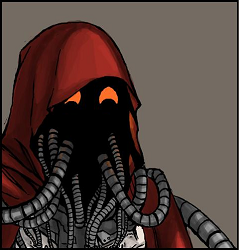
\includegraphics[width=\figwidth]{pics/7/18.png}
	\end{center}
\end{wrapfigure}
As Twitch went about disarming the explosives he gave the rest of us a pretty detailed critique. 
The bombs had been there for a fairly long time, were set up for remote detonation, and had been installed by someone who was nowhere near as good as Twitch. 
A little thinking led us to believe that the explosives had been placed by someone fairly familiar with the ship, but not with blowing things up. 
Also there were probably a few more bombs around, otherwise why bother with the remote detonator? 
While Twitch finished removing the explosives Sarge called the acolytes and explained the situation.

Jim and Hannah were pretty impressed by the discovery and the call was quickly kicked upstairs. 
Then their superiors kicked us upstairs again and again, until finally we were talking to the ever unresponsive head tech-priest; 
the Cogtain, as it were, of the horrible death-trap we were all flying on. 
For the fifth or sixth time Sarge explained that SOMEONE HAD MINED KEY COMPONENTS OF THE SHIP WE WERE ALL ON AND IT MIGHT BE A GOOD IDEA TO DO SOMETHING ABOUT IT. 
The Cogtain did not dignify us with a response and instead rattled off a bunch of binary at the other tech-priests on the line. 


There was a lot of the stupid cogboy screeching, and it sounded like they were taking the situation fairly seriously. 
None of them told us anything though. 
Eventually we got tired of them talking over our heads and Sarge suggested that perhaps the resident demolitions expert should look into the matter. 
Maybe Twitch and his good buddies, you know the guys who found the bombs in the first place, should check out the other Gellar Field Generators and Engines and such. 
This actually got a response. 
A horribly distorted voice told us to stand down and stay away from his machines, and then we were disconnected from the channel. 
That’s gratitude for you.

About ten minutes later a massive series of explosions shook the ship. 


Bloody tech-priests.

\begin{wrapfigure}{O}{\figwidth}
	\begin{center}
		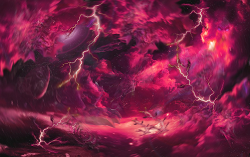
\includegraphics[width=\figwidth]{pics/7/19.png}
	\end{center}
\end{wrapfigure}
Now we knew a fair bit about explosions, every veteran guardsman does, and we were pretty damned sure that five bombs the size of the one we just defused had gone off. 
To us that suggested that the explosives had all been linked to go off when someone screwed up while defusing one of them, so chances were that the ship was down a few cogboys and major systems. 
We weren’t really concerned about that first point, but the second was worrying. 
Depending on which systems had gone down we were in for a whole spectrum of unpleasantness ranging from sudden fiery death, to less sudden chilly death, to lingering insane death. 
Sarge decided that it was probably a good idea to figure out which one we were headed for.

While the rest of us got our weapons ready Sarge tried to comm the two acolytes. 
The contact code for Jim still wasn’t letting us through, whatever the Cogtain had done to kick us out seemed fairly permanent, but after a few tries he was able to get a hold of Hannah. 
The poor cog-girl was not cut out for this stuff and sounded like she was on the brink of tears, luckily Sarge knew how to deal with shell-shocked rookies and with Doc’s help managed to calm her down enough to get a status report. 
The news was not good.

The Gellar Field Generators that covered the gaps in the top and bottom decks were completely destroyed, and both the fore and aft ones were damaged. 
Only the Generator we were sitting on and the one up near the bridge were undamaged, and between them and the two slightly damaged ones there was just enough coverage to keep the whole ship from turning into a miniature daemon world. 
It was still a very bad idea to stay in the warp any longer than necessary. 
When Sarge asked Hannah how soon we were dropping out of the warp to do repairs the poor girl dissolved into tears and broke the real bad news: 
the Warp-Drive was offline.

\begin{wrapfigure}{O}{\figwidth}
	\begin{center}
		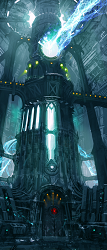
\includegraphics[width=\figwidth]{pics/7/20.png}
	\end{center}
\end{wrapfigure}
The Warp-Drive was the insanely complex device that moved the ship from boring, empty, die-of-asphyxiation-or-starvation space to horrible, daemon filled, die-insane-and-choking-on-your-own-intestines warp-space. 
Of course the whole point of this is that there are much higher speed limits in the warp or something, what’s a little daemonic incursion if it lets you get there faster right? 


Well that is a little unfair: 
the difference between a two hundred year and two week journey is pretty significant, but we were understandably bitter about the whole thing. 
The problem was that if your Warp-Drive breaks down while you’re IN the warp you don’t just pop back into reality, noooo you’re stuck there until someone fixes it. 
IF they can fix it that is, otherwise you might as well skip right to the insanity, cannibalism, and daemon worshipping and save a little time.

Things were bad, but they could have been worse. 
We weren’t dead yet, we had a moderately functional Gellar Field, the Plasma Engines were still running fine, and we were damn well going beleive that the Warp-Drive was repairable unless the Emperor himself showed up and told us it wasn’t. 
We got our shit together, armed the lethal perimeter defenses, and put up a few signs to warn anyone that trying to get near the Gellar Field Generator without our help was just a very painful method of suicide. 
We were going to hike our asses down to the Warp-Drive and take a look at it in person, because as far as we could tell no one else here was competent enough to do it. 


Of course none of us had any idea how to fix a Warp-Drive or even what one looked like, but we weren’t going to let some minor thing like that stop us.

\begin{wrapfigure}{O}{\figwidth}
	\begin{center}
		
\includegraphics[width=\figwidth]{pics/7/21.png}
	\end{center}
\end{wrapfigure}
That’s not to say that we didn’t understand the limits of our knowledge or skills. 
None of us were going to try and fix the machinery ourselves unless we had to, we’d simply start grabbing tech-priests and throwing them at the problem until they fixed it. 
Now we were perfectly aware that the Cogtain and the rest of the techies were probably trying to fix the problem, but they really hadn’t impressed us with how they handled the explosives. 
We felt that a little oversight from the few people on board who hadn’t had the “common sense” part of their brain replaced with a little box of screws might help things along.

Our first instinct was to grab one of the acolytes; 
unfortunately Hannah had been near a blast and was trapped in a room up in the bow of the ship, and we still couldn’t contact Jim. 
We didn’t really have to time to go retrieve either of them, so we figured that we might as well just shanghai the first tech-priest we came across. 
Prior to everything hitting the fan Doc had spotted a cogboy bossing around a bunch of servitors a few bays back towards the rear of the ship, and he remembered that the tech-priest had been doing something vaguely repair-like to a large conduit. 
This sounded like a good candidate for fixing the Warp-Drive, so we lined up behind Doc and went off to see if the techie was still there.

We made it to the bay where Doc has seen the tech-priest pretty quickly, we’d mapped the whole area earlier and nothing nearby was damaged. 
Unfortunately all we found inside was a horrible smell and partially opened conduit that was helpfully labeled “Dead Felid Inside, Do Not Open,” but the far door was open and so was one in the next room. 
The cogboy had obviously been in a rush to get somewhere, he’d even cut through some of the thinner bulkheads, and since he seemed to be going towards the area where the Warp-Drive was located we decided to follow his trail.

\begin{wrapfigure}{O}{\figwidth}
	\begin{center}
		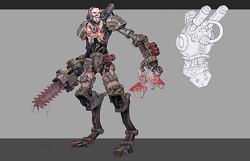
\includegraphics[width=\figwidth]{pics/7/22.png}
	\end{center}
\end{wrapfigure}
We made good time following the path the tech-priest had blazed, but the farther we travelled the more uneasy all of us felt. 
Twitch swore that someone was following us, Doc thought he heard other squad members whispering, and the rest of us were just generally uncomfortable. 
It became apparent that we were leaving coverage of the undamaged Gellar Field; 
from here on out shit was going to get spooky. 


Reality was actually pretty stable where we were, but the minor fluctuations definitely weren’t fun. 
Mostly it was little sounds or flashes of movement at the edge of our vision, and occasionally one of us would feel a flash of rage or paranoia. 
It was easy to get distracted, but Sarge kept us focused and nothing really bad happened until we caught up with the tech-priest and his servitors.

Cutter was on point, and as he entered a doorway a servitor lunged at him with a welding torch. 
Luckily, he had his chainsword ready and easily parried the blow then returned the favor. 
At that point several more servitors lurched forward, and in a rare burst of sanity our melee specialist leapt backwards out of the doorway. 
The second he cleared the line of fire, the rest of us began pouring las-fire into the approaching servitors.

These weren’t combat servitors, thank the Emperor, but they were still damned hard to kill. 
Even with the hotshot lasguns Nubby had gotten for us, it took a headshot or several joint shots to put each one down. 
Worse, they definitely didn’t have any morale to break, the horde just kept advancing with glowing eyes and sparking tools. 
We mowed down them without any getting through the door, though near the end one of them cut through the wall and barely missed Twitch.

Once we were sure that they were all dead, which was remarkably easy since all of their eyes stopped glowing with daemonic light when you finished them, we advanced into the room. 
We figured that the puddle with all the chunky bits in it was probably the tech-priest we were following. 
So much for having him repair the Warp-Drive.

\begin{wrapfigure}{O}{\figwidth}
	\begin{center}
		
\includegraphics[width=\figwidth]{pics/7/23.png}
	\end{center}
\end{wrapfigure}
It wasn’t a total loss though, the cogboy had booted up a communications console before he died and we’d definitely learned a few things about the state of the ship during our little chase. 
Mostly that servitors could be possessed or something and a weak Gellar Field meant slowly going insane, but that was still something. 
From here on out we were going to operate on the assumption that all servitors would try to kill us unless proven otherwise. 
Twitch suggested we follow the same rule for tech-priests, but was vetoed since we’d probably need a few a of them alive to get things fixed.

The console the former tech-priest had warmed up for us was waiting for input, so Sarge decided to call the Cogtain and tell him we were heading towards the the Warp-Drive to lend assistance. 
In retrospect this was a horrible idea. 
None of us had really expected him to be helpful, but we were sort of hoping he’d understand that a squad of well-trained soldiers would be an excellent escort for one of the nearby tech-priests, and maybe point us towards them. 
Instead we just got a burst of binary and a distorted screech telling us not to desecrate his machines and to let the servitors fix the problem. 
Sarge tried to explain the servitors appeared to be possessed and were not likely to be fixing anything, but all that got was a second screech that sounded an awful lot like “Ignorant Meatbags” and then the console locked us out. 
Bloody tech-priests.

Before this we’d been operating on the usual assumption that the local leadership was moderately incompetent, but after that little tantrum we decided to upgrade them to pants-on-head retarded. 
This meant that as far as we were concerned Sarge had operational command, and we weren’t even going to try talking to the senior techies anymore. 
The only way we’d start listening to them again was if they showed up with a lot more firepower than we could muster. 
That decided, we headed towards the Warp-Drive.

\begin{wrapfigure}{O}{\figwidth}
	\begin{center}
		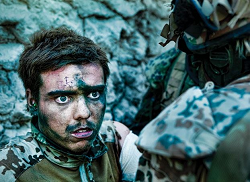
\includegraphics[width=\figwidth]{pics/7/24.png}
	\end{center}
\end{wrapfigure}
Aside from the little warpy annoyances the rest of the trip wasn’t too bad. 
Mostly it was just a matter of navigating the maze of corridors, reading the helpful notes, and dodging the occasional group of servitors. 
They all seemed to be headed towards the top of the ship, which was a little odd, but it made them easy to avoid. 
Unfortunately we didn’t run in to any other tech-priests during the walk, so when we finally got the the Warp-Drive there wasn’t much we could do.

The drive was obviously in bad shape: 
about a third of the room had been destroyed by the explosion and there were some pretty big pieces of shrapnel sticking out of the big glowy pillar thing. 
We couldn’t help but notice the lack of servitors fixing things, which pretty much proved our theory about the Cogtain’s competence or lack thereof. 
On the bright side there weren’t any servitors around to try and kill us, so it was easy to set up a perimeter around the Drive-room.

Of course we still needed to find someone to fix the damned drive, so Sarge ordered Twitch to hold the fort while the rest of the squad went off to search for a tech-priest. 
We got pretty lucky with that; 
the fifth room we checked had two of them in it. 
Well not really two, more like one and a bit, well bits, yeah… lots of little bits. 
The important thing though was the living tech-priest was Jim!

The acolyte was trying to put his boss back together like a very leaky jigsaw puzzle and didn’t seem to be all there. 
Sarge and Doc knew how to deal with this sort of thing though, and before long they had Jim up and moving if still a little shaken up. 
As we led him back to the Warp-Drive he kept insisting that his orders were to clean the incense burners down near engine three; 
apparently the Cogtain would be furious if he didn’t finish before the next maintenance cycle. 
We tried to explain fixing the Warp-Drive probably took priority, but he was very insistent.

\begin{wrapfigure}{O}{\figwidth}
	\begin{center}
		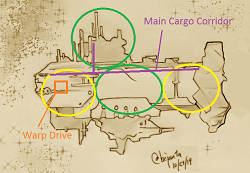
\includegraphics[width=\figwidth]{pics/7/25.png}
	\end{center}
\end{wrapfigure}
When logic didn’t work Nubby took a stab. 
He wheedled, cajoled, and outright lied to the distraught cogboy. 
See we were actually working on the direct orders of the Cogtain, and he said it was very important that we fix the Warp-Drive and every tech-priest was supposed to help us. 
In fact he had specifically said Jim should fix it because he was very impressed with all the techy things that Jim had been doing. 
Also, no, he shouldn’t call the Cogtain to make sure. 
The Cogtain said he was very busy doing things with machines and servitors and stuff. 
To everyone’s surprise Jim accepted this complete load of horseshit and started poking at the damaged drive.

Of course Jim was just a low level acolyte and knew very little about Warp-Drives, but there were quite a few of the helpful little notes around. 
He was able to pinpoint several broken components that he knew how to fix, but unfortunately some of those fixes would require rare and expensive parts. 
Parts that were so rarely replaced that no spares had been included in the ship’s inventory.

Now this sounds really bad at first, but after you spend some time in the Guard you learn the difference between what’s officially in the inventory and what’s available if you’re willing to get out a crowbar. 
Nubby got a full list of parts from the boy then went through each one and quizzed the acolyte about what other ship’s systems might use them. 
Some were pretty much unique to the Warp-Drive, but it turned out that most of the really important ones were also used in Gellar Field Generators.

We got out our map, plotted a route, gave Jim a pistol, and went to make a supply run.

\begin{wrapfigure}{O}{\figwidth}
	\begin{center}
		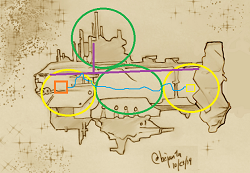
\includegraphics[width=\figwidth]{pics/7/26.png}
	\end{center}
\end{wrapfigure}
The first step of our shopping trip was deciding which Gellar Field Generator to plunder. 
The best candidates for scavenging the parts we needed in one go were the intact generators in the middle of the ship up near the bridge. 
Unfortunately, those parts were rather critical and ripping them out would probably break either generator. 
Since those two undamaged generators were probably all that was keeping the ship in reality, we opted to try our luck with one of the damaged ones instead. 
The one in the rear of the ship was right out, we needed the engines and Warp-Drive to stay daemon-free, so really the only option was the generator all the way at the bow of the ship. 
It was going to be a long walk.

In an effort to speed up our journey, we decided to divert to the big spinal freight corridor that ran the length of the ship. 
As we made our way upwards, we reached the ragged the edge of the Gellar Field’s coverage, and every one of us began to feel reality’s grip weakening. 
Cutter’s sword started talking to him, Doc’s teeth began to itch, Nubby could feel his old legs, and when Sarge and Twitch opened a door they saw a headless corpse and a charred skeleton playing poker. 
Neither of them seemed unfriendly, but we still elected to go around that room. 
When we reached an entrance to the big corridor Twitch and Jim opened up a small viewport and scouted the place. 
They closed it very fast.

According to them the corridor was packed with glowy-eyed servitors and they were all working on something. 
Twitch also spotted a few minor daemons which seemed to be randomly split between fighting the servitors, helping them, and staying out of their way. 
None of us knew what to make of that, but it was pretty clear that the main corridor was now possessed servitor territory. 
We resigned ourselves to a long, slow hike and headed back down into the ship.

\begin{wrapfigure}{O}{\figwidth}
	\begin{center}
		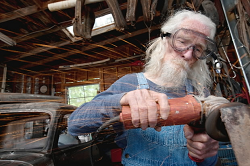
\includegraphics[width=\figwidth]{pics/7/27.png}
	\end{center}
\end{wrapfigure}
Mostly the trip was boring. 
The novelty of the ship’s horrible design had worn off long ago and we got used to the minor warp phenomena pretty quickly. 
Seen one room with faulty gravity or walls that wept blood, seen ‘em all. 
It was nice when we got into the coverage of the fully functional Gellar Field; 
we actually stopped and took a lunch break at our old base in the generator room. 
While we ate, Twitch checked his traps and reported that no one had messed with them, and Jim walked us through identifying the parts he’d need from the sacrificial generator.

Once we were through the fully covered region things started to get dangerous again. 
We ran across a few bands of servitors that seemed to be searching the ship for something as well as the occasional minor daemon. 
None of us saw any profit in slugging it out, so we all did our best to stay quiet and avoid the hostiles. 
Thanks to Twitch and Nubby’s scouting abilities, we mostly succeeded, and the single pack of servitors and handful of daemons we couldn’t go around were easy kills. 


As we got closer to the Gellar Field Generator, we heard fighting and picked up the pace. 
The source of the noise turned out the be a group of servitors trying to get into the generator room, which someone inside was vigorously defending. 
We figured that some of the tech-priests were holed up in there and hit the servitors in the rear. 


It was a clean fight, and once Cutter had finished off the last one we cautiously made our way into the room. 
Surprisingly, it was not filled with tech-priests; 
instead it contained a mob of pale old men. 
They were armed with what looked like modified power-tools, and each of them had a few yellow notepads sticking out of their pockets.

\begin{wrapfigure}{O}{\figwidth}
	\begin{center}
		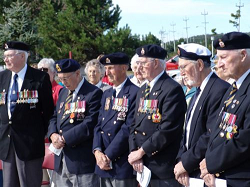
\includegraphics[width=\figwidth]{pics/7/28.png}
	\end{center}
\end{wrapfigure}
While it was a bit of a surprise to run into a bunch of stowaways, we’d sort of expected something like this. 
When the notes kept appearing we knew it was either some incredibly helpful person or some sort of warp trickery or machine spirit weirdness. 
All of us had been fervently hoping for the helpful person explanation, for obvious reasons. 
We hadn’t been prepared for just how old they were though; 
these guys looked like they were all over a hundred.

The beardiest of the stowaways greeted us all by name, which was a little creepy, introduced himself as Ol’ Bill, and thanked us for the help. 
He was apparently the leader of a group of crewmembers who hadn’t been willing to leave the ship. 
They’d outlived three captains already, and they’d be damned if they wouldn’t outlive a fourth. 
Sarge processed this, then decided to skip all the bullshit about mysteries, notes, secret passages, and all that in favor of actually getting shit done. 
He explained the situation with the Warp-Drive, our plan to rip the Generator they’d all been defending apart, and then asked the old men what it would take to get their support.

The geezers weren’t keen on scrapping the Generator, but when Jim explained the damage to the Warp-Drive they agreed that it was necessary. 
The problem was that the old crewmembers weren’t the only stowaways on the ship. 
They had a bunch of friends and even some family living in Hydroponics Bay 7C, and when the Gellar Field collapsed those folks would be ass deep in daemons. 
The old men would throw in with us if we went and evacuated everyone to a safer part of the ship, and also, just while we were in the area, got rid of the small army of servitors laying siege to the hydroponics bay.

\begin{wrapfigure}{O}{\figwidth}
	\begin{center}
		
\includegraphics[width=\figwidth]{pics/7/29.png}
	\end{center}
\end{wrapfigure}
All in all this was a pretty good deal; 
Jim was going to need some time and help getting the parts ready to be pulled and we didn’t have anything better to do. 
Before we went anywhere though we had a few things to take care of. 
While Twitch pulled out a few of his toys and beefed the Generator-room’s defences, the rest of us went to find Hannah, who was supposedly in one of the nearby damaged rooms.

We found the poor cog-girl trapped behind some rubble, and with the help of a las-cutter we pried off one of the servitors we got her out of there. 
Hannah wasn’t very happy, in fact she was practically hysterical, but she was relatively unscathed. 
None of us were well equipped to handle a panicking cog-girl, so Doc gave her a few band-aids and we unceremoniously dumped her on Jim and the old guys. 
Our heroic rescue mission successful, we gathered up Twitch and went to get the rest of the stowaways out of their hydroponics bay.

The directions that Bill gave us were great, and we quickly reached the bay’s access corridor. 
He hadn’t been exaggerating about the small army of servitors though; 
in fact it was more of a medium army now, and there were a few daemons in there too. 
They seemed keen on something inside the bay, but weren’t making much headway against the big ass doors. 
That was a good thing, because we definitely couldn’t handle all those servitors with our current loadout. 
We needed to make a plan.

We debated the problem for a while. 
Twitch was in favor of setting a large explosive trap, Doc thought there might be another way into the bay, Sarge explained to Nubby that we couldn’t just tell the old guys that they were dead when we got there, and Cutter was talking to his sword again. 
Eventually we decided to go with Doc’s suggestion and started scouting the surrounding area.

That’s how we found Hydronics Bay 9D. 
The bay that the stowaways lived in had some big warnings painted on the door: 
stuff like “Do Not Enter, Use Console To Request Rations,” “Hazardous Materials,” and “Incredibly Dangerous, Never Open”. 

9D’s door just had three meter high letters that said “BEWARE OF KNARLOC.”

\begin{wrapfigure}{O}{\figwidth}
	\begin{center}
		
\includegraphics[width=\figwidth]{pics/7/30.png}
	\end{center}
\end{wrapfigure}
Of course we didn’t believe that for a second. 
There was absolutely no reason for there to be a Knarloc on an Imperial vessel. 
It was obviously just a ruse to keep people out. 
This meant it was probably another entrance to the stowaways bay; 
with any luck we could cut through there and get everyone out without the servitors noticing.

About thirty seconds after we jimmied open the big cargo doors we slammed them shut again, because HOLY SHIT THAT KNARLOC LOOKED PISSED.

We decided to take a little breather after that scare and reconsidered our options. 
The bad news was that we definitely weren’t sneaking through that hydroponics bay, but on the other hand we had an amazing distraction available to us. 
All we had to do was get it out of the bay and down one level then it would keep the servitors busy while we snuck in. 
A little tinkering with the door controls and the nearby lift, a few dead servitors, and we were ready to rock.

It worked like a charm: 
the Knarloc barreled out of the bay the second the doors were open and ran right to the pile of servitor corpses sitting on the elevator. 
We activated the lift and watched with delight as the entire army of servitors turned to face the new threat. 
As much as we wanted to stay around and watch the fight, we had stuff to do; 
the second the last servitors left the room we dashed over to the bay’s comm panel and nicely asked them to open up.

I’m not sure what we expected to find in there, but it definitely wasn’t a flourishing tribal village in the middle of a small jungle.

\begin{wrapfigure}{O}{\figwidth}
	\begin{center}
		
\includegraphics[width=\figwidth]{pics/7/31.png}
	\end{center}
\end{wrapfigure}
Seriously, it was an entire village. 
Grass huts and everything. 


There must have been over two hundred of them in there; 
just hanging out and living a relatively simple agricultural life in the middle of a bloody spaceship. 
We’d seen weirder things, hell we’d just started a fight between a spacefaring dinosaur and a bunch of possesed mechanical corpses, but this was definitely one of those special memories that would stay with us.

It was remarkably easy to get them evacuated, this wasn’t the first time they’d migrated to a new home, and Ol’ Bill had called ahead to make sure they knew the score. 
They gathered up most of their village into packs and cargo trolleys, and then we all got the hell out of there. 
As we walked, the sounds of battle echoed in the distance along with the occasional roar. 
We congratulated ourselves on our brilliant planning, and assured each other that there was no way this was going to come back and bite us in the ass.

We led the migration back to the Generator-room without serious incident. 
The tribals seemed pretty tough, and between us and their warriors we easily managed to kill the few daemons and servitors we ran into. 
Once we arrived Bill detailed a few of his men to lead them to a safer area, then invited us in to look at the preparations for pulling out the parts.

We’d expected everything to be more or less ready, they had all the tools and knowledge of the ship after all. 
It should have just been a matter of us saying it was time to go, then they’d pull everything out and that’d be that. 
Instead they gave us a bewildering briefing about what to cut, what to grab, how to carry it, and where to go. 
Then they left.

They didn’t offer to help or check if we agreed with their plan. 
Hell, they didn’t even ask if we understood everything. 
They just bossed us around, wished us luck, then left.

In the words of that ancient guardsman hero Ollanius Pius, “Why the hell is everything always our job?”

\begin{wrapfigure}{O}{\figwidth}
	\begin{center}
		
\includegraphics[width=\figwidth]{pics/7/32.png}
	\end{center}
\end{wrapfigure}
We didn’t spend too long wallowing in self-pity though; 
you get used to this sort of thing when you’re a guardsman. 


Sarge and Doc put their heads together and formed a plan, Nubby and Cutter went over the instructions we’d been given, and Twitch cleared up his traps. 
Jim had marked out what needed to be cut, what needed to be grabbed, and what order to do it in. 
All we had to do was run to safety and we were damned good at that. 
It would all be relatively simple except for the fact that the Gellar Field would be collapsing around us.

Doc and Sarge put a lot of thought into who would be carrying what. 
Nubby was the fastest one of us thanks to his augmetic legs, so he’d grab the last parts. 
Sarge and Cutter were the strongest and would handle the heavy carts. 
Finally, Twitch and Doc would keep their weapons free to cover the rest of us. 
Each of us memorized our role in the plan, reviewed the map and directions Bill gave us, and got ready to run like the daemons of the warp were pursuing us, because they probably would be.

Sarge called Jim and Bill, made sure everyone was clear, and counted down. 
We worked fast, ripping out part after part as cables sparked and alarms blared all around us. 
The second the final piece was out we barreled out of the now smoke-filled room and ran like hell. 
We got about fifty meters before we felt the Gellar Field start to fail and reality went runny around the edges.

\begin{wrapfigure}{O}{\figwidth}
	\begin{center}
		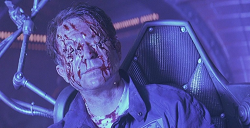
\includegraphics[width=\figwidth]{pics/7/33.png}
	\end{center}
\end{wrapfigure}
The whispers, flashes of movement, and sudden emotions hit us first. 
Doc and Twitch fired at several shadows, only one of which had an actual daemon in it, Sarge started screaming at Nubby and vowed to beat the little trooper to death with his own augmetic legs, and Cutter began apologising to his sword for not using her enough. 
We managed to keep together and keep moving though; 
even if Nubby had to take the lead since Sarge was pretty much chasing him now.

The gravity fluctuations and bleeding walls came next, along with a few more minor arcane horrors that just sort of blinked at us as we barrelled past. 
Twice we got slammed off of our feet when down changed to left or right, but we’d taken those extra few seconds to tie down the parts and didn’t lose anything. 
We did get damned messy; 
luckily warp-blood washes out just fine.

Our first serious daemon encounter came at about the halfway mark. 
Nubby came back-pedalling out a room screaming about eyes and tentacles, and we just barely managed to stop and shut the door in time. 
We tried to divert around, but both of the side passages seemed to open into the same place: 
a room which appeared to be several kilometers across and filled with fire. 
There wasn’t time for this shit, so we popped open the hatch, chucked in four grenades and one of Twitch’s detpacks, and slammed it again. 
The second the bang went off, we opened it back up and just sprinted across the room while doing our best to ignore the writhing tentacles.

We got a few rooms past that without incident then found ourselves in some sort of infinite loop of corridors. 
After the third time we passed a door, labeled “Temporary Sewage Storage, Wear a Suit,” we realized what was happening and stopped to figure things out. 
Behind us a door banged open and a mass of tentacles started pouring out.

\begin{wrapfigure}{O}{\figwidth}
	\begin{center}
		
\includegraphics[width=\figwidth]{pics/7/34.png}
	\end{center}
\end{wrapfigure}
Cutter leapt into action and started hacking off limbs while the rest of us started wildly opening doors. 
The first one had what looked like the Hospitaller and that bitch of an Interrogator tied up and screaming for help inside. 
Sarge slammed it back shut before anyone else could move. 
The second and third were filled with more tentacles and fire respectively, but we got them closed before anything bad happened. 
The next one had that headless corpse and charred skeleton playing poker again.

Now that we saw it a second time, the corpse wasn’t quite headless, he just had a bad case of exit-wound-face. 
When we opened the door he casually waved at us then rested what was left of his head on the table while his partner turned to face us. 
The well-done skeleton laughed and told us we probably wanted the the door across the hall that was labeled “Light Cargo ONLY”. 

From his resting spot on the table, the nearly-headless corpse gurgled something which prompted the skeleton to laughed again and warn us not to open the “poo door”. 

Doc awkwardly thanked him and slammed the hatch shut. 
After a brief debate we took the jolly skeleton’s advice, he seemed pretty trustworthy, and piled through the marked door. 
A second later we piled back out, grabbed Cutter, and dragged him after us.

There weren’t any side passages in the next two rooms, and when we barreled through the last door we found ourselves back in familiar territory near the edge of the safe zone. 
As we ran, reality finally started to get its shit back together and the going got significantly easier. 
We started picking up speed, only stopping to pop a few more minor daemons and divert around a pit that opened up into that huge fiery room again. 
Then, right as we started running down the last hallway, a large sword slammed through a door and Cutter immediately abandoned his cart in favor of having a sword fight with a daemon.

\begin{wrapfigure}{O}{\figwidth}
	\begin{center}
		
\includegraphics[width=\figwidth]{pics/7/35.png}
	\end{center}
\end{wrapfigure}
You could say that it was an act of heroic bravery or selfless sacrifice, but you’d be wrong. 
It was an act of complete and utter retardation, and only Sarge grabbing him by the legs while everyone else gave covering fire saved his stupid life.

The daemon followed of course, but hotshots pack a punch and we kept him back long enough for Twitch to drop a few mines. 
The second they were down we ran like little girls and just barely got around a corner before that daemon went bang. 
We didn’t go back to check if it was dead; 
as long as it wasn’t following us we were happy.

Cutter had gotten a pretty mean chest wound before Sarge yanked him away and wasn’t looking too hot as we dumped him onto one of the carts. 
Once the squad was fully inside the safe zone we stopped in a handy room and Doc got to work on him. 
While he did the stitching and stuff, Sarge called the acolytes and had them send someone to take the loot the rest of the way.

Once Cutter was sorted out we all hiked down to the Warp-Drive. 
The trip was a lot quieter this time around: 
the techies or the old crewmen must have beefed up the rear Gellar Field, and we saw a few of the tribal warriors standing guard at junctions. 
When we reached the drive-room the place was a hive of activity. 
Jim and Hannah were running around fixing things, the stowaways were acting as assistants and advisors, and Ol’ Bill was yelling directions at everyone.

The second he saw us, Ol’ Bill waved us over and filled us in. 
Repairs were going well, the perimeter was holding up fine, and it wouldn’t be long until we could shift back to real-space. 
We all breathed a sigh of relief, but before anyone could celebrate Hannah poked her head out of a gutted machine and reported that some piece warpy tech was busted. 
Everyone went quiet at this. 


Ol’ Bill thought hard for a few seconds then brightened up and told everyone not to worry: 
there was a spare aboard. 
The old bugger turned to us, gave a toothless smile, and said he needed a few brave lads to fetch a part from the Psyker Holding Cells downstairs. 
As one we turned to Nubby, who started to sidle out of the room.

\begin{wrapfigure}{O}{\figwidth}
	\begin{center}
		
\includegraphics[width=\figwidth]{pics/7/36.png}
	\end{center}
\end{wrapfigure}
You see, with the exception of Cutter, all of us had a bit of experience with psykers and ships with Psyker Holding Cells. 
We’d been part of a team which had busted up a corrupt government group that was gathering up all of a planet’s nascent psykers, usually as children, and was selling them off-world. 
That mission had ended with us being sent home with a scathing report which we then doctored to make us look better. 
Last we’d heard, the jackass who was running the investigation was still looking for the rest of the ships which had been used to transport the kidnapped psykers.

Up to this point, we’d put Nubby’s position as the ship’s procurer down to bureaucratic incompetence or a completely understandable desire to get him out from underfoot. 
From there it was easy to blame the horrible quality of the ship on Nubby’s unique weasley incompetence, as well as some of the ordinary variety from his bosses. 
All that went out the window the second we heard the phrase “Psyker Holding Cells” though, and we jumped to some new conclusions.

As we walked Sarge grilled the despicable little trooper and the truth finally came out. 
He’d spotted this ship in some report or other and instead of turning it in and having it seized the cretin had decided to try and impress his boss. 
Nubby had flagged the ship as a prospective purchase, and then went and swore up and down to his superior that he could get it at a much lower price than anyone else. 
Emperor only knows why his boss agreed. 
Possibly, the poor man had just wanted Nubby to go away for a few months.

Right up to that final meeting with the fat captain the purchasing process had gone normally. 
Then Nubby, in his infinite brilliance, had told the man that he knew the ship’s dirty secret and threatened to expose him if he didn’t bring down the price.

It wasn’t hard to see why bombs had been planted on the ship or who had planted them. 
Damn Nubby and his bloody stupid schemes.

\begin{wrapfigure}{O}{\figwidth}
	\begin{center}
		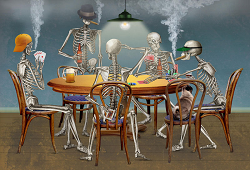
\includegraphics[width=\figwidth]{pics/7/37.png}
	\end{center}
\end{wrapfigure}
The worst part was how he tried to defend himself, pointing out that he “didn’t lie to nobody ‘bout nofink,” and “spificly said we weren’t ‘Quisitiors, an’ there weren’t no ‘ard feelins an’ it was jus’ bisness,” and “got a really good deal even wif all da dents an’ stuff”. 



We were all just about ready to kill him, and Sarge probably would have if we didn’t have other concerns at the moment. 
Instead we privately vowed that Nubby would never again be allowed any sort of authority and, if we survived this, everything would be blamed on him. 


Our trip started to get hairy as we descended deeper into the ship; 
the cells were way at the edge of the current Gellar Field coverage. 
Aside from the usual weirdness and the fair number of minor daemons, which we killed if we couldn’t avoid them, we ran into a few more of those spooky doors that opened into weird places. 
We got that huge fire room five times, the tentacle daemon twice, and found one room inhabited by some sort of sewage monster. 
That last one might have been real though, the note on the door did say “Xenos Waste Processing Device, Do Not Enter.”

The last warpy door we ran into had the rather crispy skeleton playing poker again, but now the head-shot man was slumped in an armchair in the corner and a bunch of other players had taken his place. 
We spotted a bunch of ghostly looking soldiers with regimental insignias we couldn’t quite make out, and some vague spectres who looked eerily familiar. 
The was also a big guy with a sword drowning someone wearing robes in the punchbowl. 


As we tried to quietly shut the door, the skeleton spotted us and congratulated us on staying alive. 
The nearly-headless one jerked up in its chair and gurgled something then slumped back down. 
The burnt skeleton practically fell over laughing at this, but he caught his breath right before we slammed the door. 
As the hatch closed, he advised us to check the cells before we took our part. 
A second after we’d slowly backed away from the door, it popped back open, and we heard the skeleton shout that the big guy said no hard feelings and not to open the last cell. 
On that cryptic note, the door slammed shut again.

We spent a few seconds digesting the skeleton’s advice, and how oddly familiar the room’s occupants had been. 
Twitch suggested opening it back up for another look, but Sarge vetoed this and led us down the last corridor to the psyker cells.

\begin{wrapfigure}{O}{\figwidth}
	\begin{center}
		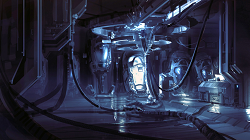
\includegraphics[width=\figwidth]{pics/7/38.png}
	\end{center}
\end{wrapfigure}
The Psyker Holding Cells were much, much fancier than anything else we’d seen on the Occurrence Border. 
It was a fairly small place, with only a dozen actual cells, but they’d obviously been custom built and installed instead of scavenged; 
it had probably been some part of the contract for hauling the psykers. 
The part we needed was sticking out of some arcane machine in the middle of the main room, right where Ol’ Bill said it would be. 
We cut open the casing, loosened the part, and left it in place while we checked what was inside the cells: 
the skeleton and his macabre buddies hadn’t steered us wrong yet 

We all got into covering positions around one of the doors. 
Doc opened it, peeked inside, and started swearing when he saw its occupant. 
The kid didn’t look more than eight years old, though who knew how long he’d been lying in that stasis field, and there was a little card at the foot of his bed which had a greek letter and a list of specialties. 
This one was apparently a pyromancer and a telekine.

We checked the rest of the cells, except for the one we’d been warned about, and found about half of them occupied. 
We had five psykers between the ages of five and ten sitting in stasis, and chances were the only thing keeping them from being possessed by big-ass daemons was the part we were about to take.

The smart option at this point would have been to just kill them. 
We couldn’t take their stasis beds with us, and we were in the middle of a freaking incursion here. 
This was just about the worst place and time to have a bunch of untrained psykers running around. 
In the end though none of us were big enough bastards to do it. 
One by one we pulled them out of their beds then, since we weren’t complete idiots, we tranqued them and stuffed them into our backpacks. 
They didn’t weigh much more than a full field kit.

For the second time that day we planned our path, yanked out a piece of delicate machinery, and ran like hell.

\begin{wrapfigure}{O}{\figwidth}
	\begin{center}
		
\includegraphics[width=\figwidth]{pics/7/39.png}
	\end{center}
\end{wrapfigure}
We didn’t have to contend with nearly as much warp bullshit this time, but the second we pulled out that part the one unopened door was dented outwards and we heard daemonic howling from every direction. 
We ran as fast as we could and kept our weapons ready.

The first few were the minor daemons we’d been seeing everywhere and it only took a single shot to put them down. 
The problem was that every one cost us a second, and SOMETHING was slamming up the corridors behind is. 
It did NOT sound friendly, but we were doing a pretty good job of keeping ahead of it at first. 
It wasn’t until we ran into the larger daemons that whatever was chasing us began to gain ground.

That damned tentacle daemon was the first one we ran into. 
It burst through a door as we were running past and made a grab for Doc’s kid. 
He dodged just in time, and Cutter managed to hold the thing off long enough for the rest of us to get past. 
For once we didn’t need to pull the nutcase away from the fight: 
the second we were clear he started falling back. 
Twitch tossed a few hot nades into the mess of tentacles which kept it back long enough for us to slam a door shut and continue our run. 
A short time later we heard some especially loud daemonic shrieks, a few clangs, and the sound of a shut door being torn open.

After that it was clear running for a while. 
There were a few of the small fry, another door with the two disguised daemonettes which we slammed shut, Nubby was nearly set on fire when his kid manifested a few small fireballs in his sleep, but it was basically easy going. 
We were getting tired though, and whatever was behind us was gaining. 
We started shutting every door we went through, and Twitch began dropping mines, but as far as we could tell that only made it madder.

\begin{wrapfigure}{O}{\figwidth}
	\begin{center}
		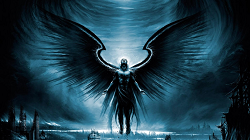
\includegraphics[width=\figwidth]{pics/7/40.png}
	\end{center}
\end{wrapfigure}
Eventually it became clear that the strengthening Gellar Field wasn’t going to stop our pursuer, so as we ran we got ready for a fight. 
The moment we ran into one of the small groups of tribal warriors we practically threw the kids on them and slammed the door we’d come through. 
We piled the last of Twitch’s detpacks plus every grenade we had around the door, then got into firing positions. 
Half a minute later the hatch burst open and a daemonhost flew though.

We thought it looked like a little kid with big black wings made of smoke, but none of us got a long look before the explosives went off. 
The second the shockwave was past, every one of us began pouring full-auto fire down the smoke-filled corridor. 
After about half a minute of continuous firing, our view began to clear and we all heard a voice in our heads vowing vengeance as soon as it found a more suitable host. 
At Sarge’s order we stayed in position for another few minutes in case it was a trick, but the daemonhost didn’t reappear. 
Eventually we declared victory and headed up the Warp-Drive to see how things were going.

Some tribal women were caring for the kids when we got there. 
Doc ran over and made sure no one tried to wake them up while the rest of us resupplied and talked to Ol’ Bill and the acolytes. 
They were overjoyed to see the part we’d got for them and immediately started welding it into place. 
While they worked Bill explained that everything was pretty much ready and all that was left to do was call up to the bridge and get whoever was piloting this thing to take us out of warp. 
All of us groaned at that.

We knew this meant talking to the Cogtain and weren’t looking forward to the conversation. 
Hopefully he’d just accept that we’d saved his bacon and hit the damned button instead of yelling about stuff. 
Hannah went over and tinkered with the room’s comm console, and Sarge got ready to do the talking.

We’d been expecting a little shouting or something. 
Instead all we got deranged voice screeching about “weak flesh” and “Avatar of the Omnissiah”. 

Then the console caught fire.

\begin{wrapfigure}{O}{\figwidth}
	\begin{center}
		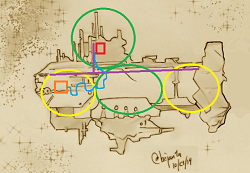
\includegraphics[width=\figwidth]{pics/7/41.png}
	\end{center}
\end{wrapfigure}
The consensus was that the Cogtain had completely lost it, so someone had to go upstairs and hit the buttons on the bridge. 
Of course everyone looked at us as they said that, it just wasn’t surprising anymore.

At least we managed to convince them that we needed a short break before we ran into another fight. 
All of us grabbed a snack and tried to catch a few minutes of sleep. 
While we rested, one of Bill’s men went and fetched the really heavy ordinance that we had left in our quarters. 
We figured that we’d need every bit of firepower we could get for this trip because the only way to access the command deck was through the main lifts located in the big spinal corridor. 
The one full of possessed servitors. 
At least we’d be crossing it where there was good Gellar Field coverage.

When our heavy weapons arrived, we staggered to our feet and got ready for one last hike. 
Twitch had all of his explosives, Sarge had his grenade launcher, Nubby had a few single shot rockets, and Doc and Cutter had as much ammo as they could carry. 
There was no way we’d cross that corridor without being noticed, so we might as well be ready to kill whatever we ran into.

We made sure we had a clean comm connection to the acolytes and clanked our way up towards the big spinal corridor. 
We planned our route so we’d spend the minimal amount of time in there before we got to the lifts and prayed to the Emperor that most of the servitors would be busy somewhere else. 
Unfortunately it didn’t work out that way: 
as we reached the edge of the safe zone a pair of tribal scouts reported that the servitors were building something almost right on top of the lifts.

\begin{wrapfigure}{O}{\figwidth}
	\begin{center}
		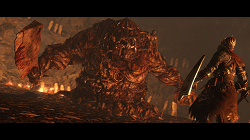
\includegraphics[width=\figwidth]{pics/7/42.png}
	\end{center}
\end{wrapfigure}
What we saw when we peeked into the big hallway was pretty damned terrifying. 
The servitors were piling all sorts of materials, including themselves, into some sort of giant structure. 
A ring of what looked like every surviving tech-priest was standing around the structure giving commands to the servitors and chanting in binary. 
Up above all this activity there was a hovering platform and standing right in the middle of it, screaming like a cross between a shorted vox unit and a mechanical sprinkler, was the Cogtain. 
Also everything was glowing, which was probably bad.

We didn’t wait to see what was going to happen or bother trying to find a way to sneak around. 
We just hefted our weapons and started pouring as much fire as possible into both the growing structure and the tech-priests. 
Metal and meat flew everywhere, our first volley tore apart dozens of servitors and cogboys, but to our surprise they didn’t react at all. 
They just ignored us while they kept chanting and building. 
We didn’t stop to ponder this; 
if they were going to hold still and be easy targets, then we were going to take advantage of it.

Unfortunately this happy state didn’t last for long. 
Before we could kill more than half the tech-priests the chanting rose a crescendo, and the surviving cogboys climbed onto the structure with the last of the servitors. 
The Cogtain stepped off his platform onto the top of the thing and with a slow smooth movement the whole damned pile stood up.

It was like some sort of servitor titan, and boy was it pissed.

\begin{wrapfigure}{O}{\figwidth}
	\begin{center}
		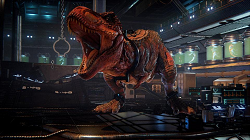
\includegraphics[width=\figwidth]{pics/7/43.png}
	\end{center}
\end{wrapfigure}
We poured the rest of our launcher rounds and missiles into the damned thing without much effect. 
A few servitors dropped off, but the others sort of flowed into the holes and the thing just kept coming. 
As it approached, the Cogtain kept up his screaming and added the occasional gothic insult. 
We decided it was time to get the hell out of there and turned towards the door we came through.

Right as we got to it there was an especially loud screech from behind us, and the door slammed shut. 
Then the door on the other side of the corridor slammed shut. 
Finally, with a tremendous crashing sound, every door down the length of the corridor shut itself. 
We took a look at the doors, then at the servi-titan, briefly pondered the situation, and started running down the corridor like scared little girls. 
Behind us the monstrosity lengthened its gait and started picking up speed.

As we ran we dodged past a few remaining servitors and minor daemons who wandered towards the titan. 
We didn’t stop to worry about them, but when we looked back the monstrosity was stopping to pick them up and slap them into its body. 
That was probably a bad thing, but at least it was slowing the monster down.

We started to gain a lead on the servi-titan and began considering options. 
We were down to shooting it a lot and hoping it had a weakpoint, piling all of our explosives together and hoping it was enough, or blasting open a door. 
Sarge decided to go with the big pile-o-mines, but just as we were getting ready to stop and set it up we saw something ahead of us.

Something about as large as the servi-titan was coming down the corridor. 
On closer inspection it appeared to be some sort of large bipedal lizard. 
With wings. 
Black smoky wings. 
Also horns and very glowy eyes.

\begin{wrapfigure}{O}{\figwidth}
	\begin{center}
		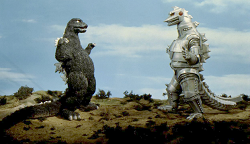
\includegraphics[width=\figwidth]{pics/7/44.png}
	\end{center}
\end{wrapfigure}
So no shit there we were, trapped in a hallway with a horrible servitor titan coming at us from one side and a possessed Knarloc coming from the other. 
There were probably worse positions to be in, but damned if we could think of any at the moment. 


Suddenly blasting open a door looked like the best available option. 
We all unhelpfully yelled at Twitch as he picked out a small door and set the minimum number of charges needed to open it up. 
Both the daemonic horrors were closing on us as we took cover and hit the detonator. 
It was all we could do to stay in cover until the explosives went off. 
The second the door was open we piled through and got as far away from it as possible.

Behind us there was a loud crash, and a good portion of the bulkhead around the door bent inward. 
A second later there was a meatier sounding crash and a tremendous amount of screeching and roaring. 
We all watched the doorway as huge feet stomped back and forth and the noise continued. 
From the look of things the two monsters had gotten into a bit of a fight, and for the time being we’d been forgotten. 


We had absolutely no desire to interrupt that fight; 
it was the only distraction we were likely to get and hopefully one of them would kill the other. 
We ran along side rooms and passages as quickly as we could and got as far towards the lifts as possible before we blew open another door. 
As soon as it was open we started running down the corridor as fast as our legs could carry us. 
Every once in a while we’d look back to make sure the giants were still fighting and hadn’t noticed us.

Amazingly our luck held out and we reached the elevators without incident. 
We piled onto the single large platform that would take us up to the bridge, hit the button, and breathed a sigh of relief as the fight dropped out of sight.

In an offhand way Twitch wondered if the fight would end with them combining into a daemoni-servi-knarlo-titan. 
No one laughed.

\begin{wrapfigure}{O}{\figwidth}
	\begin{center}
		
\includegraphics[width=\figwidth]{pics/7/45.png}
	\end{center}
\end{wrapfigure}
As we rode up, Sarge commed Jim and the rest to make sure everything was still okay and fill them in on the situation. 
The acolytes took the news about the Cogtain a little hard, but otherwise everything down there was just fine. 
All we had to do was hit a few buttons and we’d be out of the warp. 
Down below us there was a titanic crash and a scream that shook the walls. 
Nubby pushed the up button a few more times, and Twitch started getting the rest of his explosives ready.

When we reached the top of the elevator, Twitch fixed his detpacks to platform’s joints, and we all headed through a pair of impressive looking doors. 
The bridge was large, filled with blinking lights, had a massive but slightly cracked window that was currently covered, and was practically papered with little yellow notes. 
As we stood and pondered the massive array of buttons there was another scream, and the elevator started to descend. 


That focused our attention nicely, and we started hunting through the arrays of controls for the Warp-Drive switch. 
Bill had said it was large, blue, labeled “Fire Missile Bay 26F,” and had a note that said “Never Ever Ever Touch”. 

That last part was completely useless, almost every note on the bridge said that, and we wondered how the Cogtain had steered this thing. 
Maybe he just jammed his tentacles into it or something.

It took a fair bit of painful trial and error to find the right switch. 
Every time one of us found one that looked good we hit it and hoped for the best. 
Before we got the right one we managed to find the controls for three cargo bays, a positioning engine, and the gravity for the top third of the ship. 
That last one nearly killed us, but Doc managed to hold onto it and get it back to normal before anyone got badly hurt.

When we finally found the right switch we flipped it down and waited for something to happen. 
There was a charging sound, an incredibly loud *CLANG*, and Jim helpfully informed us that a major daemonic presence was keeping us from dewarping.

\begin{wrapfigure}{O}{\figwidth}
	\begin{center}
		
\includegraphics[width=\figwidth]{pics/7/46.png}
	\end{center}
\end{wrapfigure}
It didn’t take long to guess what was going on, and we all ran to the elevator shaft and looked down. 
Twitch started giggling as the daemoni-servi-knarlo-titan slowly rose towards us.

The thing looked pretty mean. 
Well actually it looked pretty much the same as it had before, except with a  Knarloc head for an arm and an undersized set of smoky wings. 
Still, that was way more than we wanted to fight. 
Sarge gave Twitch a poke, and the trooper hit all of his detonators.

The platform disintegrated along with the bottom half of the monstrosity, but as we all watched in horror the thing sank its claws and teeth into the side of the shaft and began to climb. 
This was not a good thing: 
we had no desire to fight this horror in close combat. 
We got out our lasguns and grenades, and every one of us poured as much fire as possible into the thing’s hands.

The monstrosity made it about three quarters of the way up to us before, all at once, its normaller hand disintegrated. 
The thing managed to hang on with its dino-arm for a moment then plummeted down into the depths. 


A few seconds later there was an impressive squishing sound, then the universe went “prolg” and tasted faintly of the color yellow. 
We all turned and watched as the large shutters on the bridge’s front window started to open. 
The Occurrence Border had achieved reality.

As we congratulated each other on a job well done and wandered back towards the bridge there was an ominous swooping sound behind us. 
All of us turned to face the shaft and watched the Cogtain rose out of it; 
complete with smoky black wings and curly metal horns. 
No one moved, not us and not the daemonic tech-priest, everyone just stood there and calculated the odds.

Then Cutter revved his chainsword, the Cogtain let out a horrible screeching laugh and hefted his gear-staff, and both of them lunged forwards.

\begin{wrapfigure}{O}{\figwidth}
	\begin{center}
		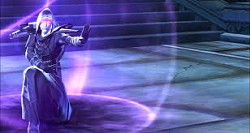
\includegraphics[width=\figwidth]{pics/7/47.png}
	\end{center}
\end{wrapfigure}
Each of us sprang into action like the pros we were. 
A torrent of las-fire plowed into the daemonhost, and Cutter neatly intercepted his charge. 
He met the Cogtain’s staff with his chainsword, forced the stroke aside, and then dodged away so we could get another volley in.

We repeated this trick three times before the daemonhost let out a scream of frustration and leveled his staff at Doc. 
A bolt of black lightning hit the medic in the chest and threw him into a wall, but before the Cogtain could follow up his attack Cutter brought his sword down and removed one of the bastard’s metal arms. 
Unfortunately he didn’t manage to dodge the Cogtain’s counterstroke and was thrown nearly to the edge of the shaft.

With Cutter out of the line of fire, the rest of us poured as much las-fire as we could into the daemonhost and actually started to force the foul thing back. 
He countered with a few more lightning bolts, but two missed their mark and the last one only fried one of Nubby’s legs. 
We managed pushed the Cogtain all the way to the edge of the shaft where he crouched and put up some sort of shield. 
Behind him Cutter silently got to his feet and raised his sword

\begin{wrapfigure}{O}{\figwidth}
	\begin{center}
		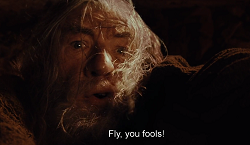
\includegraphics[width=\figwidth]{pics/7/48.png}
	\end{center}
\end{wrapfigure}
Cutter didn’t manage the decapitation he was aiming for, but he got one of the smoky wings and knocked the Cogtain off balance. 
A few shots from the rest of the squad pushed him a little farther, and the daemonhost slowly began to topple into the shaft. 
At the very last second his remaining hand reached out, grabbed Cutter’s ankle, and pulled it out from under him.

Cutter just barely managed to grab the edge of the shaft with both hands and kick off the Cogtain’s grip. 
The daemonhost started to erratically fall down the shaft, flapping his remaining wing and screaming curses in a horrible mix of daemonic and binary. 
Cutter didn’t spare any attention for the falling Cogtain, he was fixated on something much more important. 
Next to him, just barely out of his reach, his chainsword was teetering on the lip of the shaft. 
He watched in horror as, ever-so-slowly, it tipped over.

Sarge saw what was coming next and almost managed to get there in time, “almost” being the key word. 
The damned fool let go of the edge and swung himself towards his beloved chainsword. 
The noncom watched as Cutter made the catch then dove like a falcon onto the flailing daemonhost. 
He wrapped his legs around the Cogtain, raised his rescued sword, and started hacking at the metal bastard while screaming at the top of his lungs.

\begin{wrapfigure}{O}{\figwidth}
	\begin{center}
		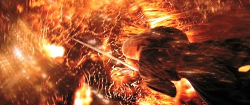
\includegraphics[width=\figwidth]{pics/7/49.png}
	\end{center}
\end{wrapfigure}
Sarge and Twitch stood there and watched Cutter fall toward his heroic death, but Nubby, bless his blackened little heart, sprinted as fast as his damaged leg could carry him back towards the bridge.

About five seconds before Cutter and what was left of the Daemonhost hit the ground Nubby found the gravity control and threw it in the opposite direction. 
Sarge, Doc, and Twitch all slammed into the ceiling; 
collecting a concussion, four broken ribs, and a dislocated shoulder between them. 
Meanwhile a rather bewildered Cutter flew back up the shaft on a very injured daemonhost.

It took Nubby a few tries to get the gravity just right, but eventually he zeroed it out, and Cutter managed to flail his way to safety. 
As soon as he was clear Nubby cranked up the gravity as high as it would go, and the Cogtain flew down the shaft at incredible speed. 
Later we checked the bottom of the elevator shaft. 
He punched through four decks and half of an awkwardly placed wall before he stopped. 


We set up camp in the bridge. 
Doc had a nasty burn but would be okay, there were a lot of minor broken bones, and Cutter had an impressive series of cuts all over his chest, the Cogtain hadn't gone down easy. 
We were all still alive though, and based on what Jim and Bill told us the ship was in relatively stable condition. 
As long as you ignored the massive warp taint in the bow and the upper and lower decks that is.

We called that a victory and stood the hell down.

It took them a day and a half to rig up a replacement elevator, but we didn't notice. 
We were busy sleeping.

\begin{wrapfigure}{O}{\figwidth}
	\begin{center}
		
\includegraphics[width=\figwidth]{pics/7/50.png}
	\end{center}
\end{wrapfigure}
Getting the ship back in, well, ship-shape was a lot of work, but easier than it might of been. 
For instance, we might have lost the Navigator and Astropath who steered our ship in the warp and enabled interstellar communications respectively.

We found the the Navigator alive and well, he’d apparently been following the standard Navigator operating procedure for a warp incursion. 
Said procedure was to just lock yourself in your sanctum and ignore all the daemonic silliness while you concentrate on steering the ship through the warp. 
A remarkably sane response all things considered, and about the same as the one the Astropath had been following. 
Except in the Astropath’s case he wasn’t keeping the ship from crashing into a reality reef: 
he was just hiding under his bed and crying. 
We left the Navigator to his business and pulled the Astropath out then made him send a report along to Oak.

Telling your boss that you are going to be late for work because ninety-nine percent of your Mechanicus contingent had been possessed by daemons and subsequently purged is very awkward. 
Sarge tried to mitigate the unpleasantness of the situation by blaming everything on the Cogtain, it’s not like the guy was in any condition to argue. 
That worked to a certain degree, but we still wound up being very thankful for the slow and unreliable nature of Astropathic communication: 
it saved us explaining the situation in detail as well as the scathing lecture Oak doubtlessly would’ve given in return.

Anyway, those two psykers were the only irreplaceable components on the ship: 
Ol’ Bill loudly claimed that given enough time and duct-tape he could fix everything else. 
Jim and Hannah were dubious at first, but the next few weeks proved the elderly engineer right.

\begin{wrapfigure}{O}{\figwidth}
	\begin{center}
		\includegraphics[width=\figwidth]{pics/7/51.png}
	\end{center}
\end{wrapfigure}
The next few weeks were educational. 
Also infuriating, exhausting, and occasionally scary, but mostly educational.

First, we learned how pragmatic engineers deal with sections of ship that have been warp-tainted or only get sporadic gellar-field coverage: 
you ignore them. 
Well not exactly ignore, you still have to go through the effort to wall off the area and make sure nothing is living in there. 
Ol’ Bill claimed that as long as there was nothing to possess and no way for warp-entities to get into the rest of the ship it worked fine; 
at least until you could come in later and cut out the whole tainted section. 


All of us were a little dubious, but Ol’ Bill said he’d done the procedure several times before. 
In fact all those incidents where the “front fell off” had been the application of this method of damage control on a large scale. 
He even suggested that if the shipyard was squeamish about the cost of doing a cut-and-refit he knew a handy trick involving carefully lowering the void shields near a star. 
We pondered the melted look of the Occurrence Border’s prow and decided the man probably wasn’t bullshitting us.

After that we learned just how many krootoid creatures had been living in the hydroponics bay with that Knarloc. 
Apparently the previous captain had decided that having a Kroot mercenary aboard would make him seem more Rogue Traderish. 
Of course when the xenos had the gall to demand payment, it’d been ditched on a planet. 
The Kroot’s pets were harder to clear out though, and the bay had eventually been sealed in the hope that they’d eventually starve. 
They hadn’t, in fact they’d multiplied, and after we’d opened the bay they’d flooded into every corner of the ship. 
The job of hunting every beaked-beastie out of a section before it was sealed fell to us and some of the tribals. 
It was rather disconcerting how many had started to mutate by the time we found them.

Finally, we learned that, despite it’s size, it only really took about fifty crewmen to fly the Occurrence Border, if you didn’t have to worry about cargo hauling or complex life support systems that is. 
We managed to scrape up enough hands, but it was a close thing and all of us were kept incredibly busy. 
At least we weren’t stuck with caring for those psyker kids though, that job fell to some of the tribal women and the useless Astropath. 
Doc checked in on them occasionally and said they were doing fine. 
The rest of us took his word for it, and stayed as far away as possible.

\begin{wrapfigure}{O}{\figwidth}
	\begin{center}
		\includegraphics[width=\figwidth]{pics/7/52.png}
	\end{center}
\end{wrapfigure}
When the repairs were finished, our journey to the shipyard resumed. 
Out of necessity we kept the warp jumps short and the Navigator stuck to only the stablest and best-mapped warp-currents as opposed to the fastest ones. 
It took a good deal longer than what had originally been scheduled to get to our destination, but we did get there in the end. 


Once the Occurrence Border was finally in its dock, a shuttle came and took us into the shipyard. 
While it was an incredible relief to get off that deathtrap and onto a nice, solid station, the whole thing was rather ruined by the fact that one of Oak’s personal retinue was waiting there for us.

The report didn’t go over as badly as we’d feared: 
Oak’s assistant was more incredulous that furious. 
Every part of our story, from the ship’s purchase to the Cogtain’s possession, was met with a sort of baffled exasperation from the man. 
It wasn’t until we brought him to the ship and showed him the ungodly mess at the bottom of the elevator that he started believing us.

Despite our earlier promise to pin everything on Nubby, we did our best to put a positive spin on his part in things. 
Of course in this case “positive spin” meant twisting the truth into decorative little knots to paint his behavior as mere incompetence. 
Y’know, as opposed to a deliberate subversion of Inquisitorial justice in an attempt to score a cheap ship and look good for his boss. 
In the end Nubby was fired from his job in supply, which was good, and reassigned back to active duty as part of the squad, which was also good. 
So all that worked out pretty well.

Once we’d convinced Oak’s assistant that everything wasn’t our fault, we were able to spare some concern for our fellow survivors. 
Luckily, the man didn’t turn out to be the sort of Inquisitorial agent who liked ordering mass-executions after every little incident.

\begin{wrapfigure}{O}{\figwidth}
	\begin{center}
		\includegraphics[width=\figwidth]{pics/7/53.png}
	\end{center}
\end{wrapfigure}
Jim and Hannah were given a lot of praise for fixing so many things and not going all crazy like every other damned tech-priest on the ship. 
Oak’s assistant talked to some senior tech-priests at the shipyard, and the acolytes were given some papers which said they’d officially finished their apprenticeship and were being seconded to the Inquisition for their first independent assignments. 
We welcomed them to the team and wished them luck with their first Interrogator.

All of us had been pretty sure the tech-acolytes would come out fine, but we’d been a bit more worried about what would happen to Ol’ Bill, his band of un-retired crewmen, and the hydroponics tribe. 
We needn’t have though: 
they were all just accepted as part of the ship. 
Both Oak’s assistant and the yard’s tech-priests said that most ships had permanent inhabitants, and as long as they didn’t get in the way they’d just become part of the next crew. 
In our opinion it was rather cruel to leave them on that horrible ship after all they’d done, but Ol’ Bill and the rest seemed happy with the result. 
We didn’t kick up a fuss and wished them all luck.

Finally the half-dozen psychic kids we’d rescued were bundled off to whatever place the Inquisition sends powerful young psykers. 
Oak’s assistant seemed to think that they were the one bright spot in all this mess, and said their “acquisition” would do a lot to smooth things over with the boss. 
We took that as a sign that the creepy little buggers weren’t just going to be shot and didn’t speculate on whether being raised by the Inquisition was any better.

As for the Occurrence Border itself, the folks working on it said it was definitely repairable. 
Sure, it was going to take a year of intensive work to get it livable again, but it would fulfill its intended purpose as a disguised Inquisition transport wonderfully. 
Honestly we didn’t give a damn what happened to the horrible deathtrap. 
As long as we never had set foot on it ever again we’d call anything a victory.

\begin{wrapfigure}{O}{\figwidth}
	\begin{center}
		\includegraphics[width=\figwidth]{pics/7/54.png}
	\end{center}
\end{wrapfigure}
Once all the loose ends were tied up, we were packed onto a ship with Oak’s assistant and rode back in relative peace. 
No one told us to do things, no one interrupted our sleep, and the only tech-priests around were Jim and Hannah. 
It was quite relaxing, and we were in good spirits when we reached Oak’s ship.

Nubby was called down to his end of the ship for an official firing before he was sent back to us. 
Twitch and Cutter hauled the acolytes down to our regiment’s section of ship and showed them off like proud parents. 
Doc wandered off to a certain medical section of the ship and wasn’t seen for several days. 
When he finally got back the poor boy looked utterly exhausted, but he seemed happy.

Sarge was called down to Oak’s office. 
Not the whole squad, just him. 
Everyone speculated about what was going on in there; 
maybe Oak was really pissed at us this time, or maybe he was going to force Sarge to accept a promotion. 
In the end our fearless leader marched back out with a glazed expression and went straight to the bar. 
A few drinks later we got him talking: 
Oak wasn’t mad at us, and while he had hinted at the promotion he hadn’t carried through. 
The reason Sarge was called up, and why he was drinking, was because he’d already received the squad’s next assignment.

In a few months time a whole new batch of trainees would arrive. 
It was going to be our job to teach them, whether they were guardsmen, psykers, or scribes, how to be proper Inquisitorial agents. 


That was a damned tall order and no mistake... 
Hell, we didn’t know how to be proper Inquisitorial agents ourselves.

All of us sat down with Sarge and started drinking too. 
This next one was going to be weird.
